\documentclass[pdftex,11pt,a4paper]{article}
\usepackage[pdftex]{graphicx}
\usepackage{fancyhdr}
\usepackage{geometry}
\usepackage{draftcopy}
\usepackage{float}
\usepackage{amsmath}
\usepackage{algorithm2e}

\renewcommand{\thesection}{\arabic{section}.}
\renewcommand{\thesubsection}{\arabic{section}.\arabic{subsection} }
\renewcommand{\headrulewidth}{0pt}
\renewcommand{\footrulewidth}{0.5pt}
\pagestyle{fancy}
\fancyhead{}
\fancyfoot[LE,LO]{\footnotesize{
SE344, Chemistry and Our Environment
}
}

\title{\vspace{-15pt}Horizontal Gene Transfer\\ SE344: Chemistry and Our Environment}
\author{Ankesh Kumar Singh (Y9090)}
\date{9th February, 2013}
\begin{document}
\maketitle
\hrule
\vspace{10pt}
Horizontal gene transfer (HGT) refers to the transfer of genes between organisms in a manner other than traditional reproduction. Also termed lateral gene transfer, it contrasts with vertical transfer, the transmission of genes from the parental generation to offspring via sexual or asexual reproduction. HGT has been shown to be an important factor in the evolution of many organisms. It is useful for environmental adaptation. It Is easier to have gene transfer between virus and humans, than between a human and organisms like rats. Nature has been extremely clever in the way it has developed organisms. It has a class of common proteins that has been organized in a different manner to constitute any organism.
\vspace{5pt}\\
Horizontal gene transfer occurs in 3 ways:
\begin{enumerate}
\item \textbf{Transformation} - the uptake of naked DNA is a common mode of horizontal gene transfer that can mediate the exchange of any part of a chromosome; this process is most common in bacteria that are naturally transformable; typically only short DNA fragments are exchanged.
\item \textbf{Conjugation} - the transfer of DNA mediated by conjugal plasmids or conjugal transposons; requires cell to cell contact but can occur between distantly related bacteria or even bacteria and eukaryotic cells; can transfer long fragments of DNA.
\item \textbf{Transduction} - the transfer of DNA by phage requires that the donor and recipient share cell surface receptors for phage binding and thus is usually limited to closely related bacteria; the length of DNA transferred is limited by the size of the phage head.
\end{enumerate}
\begin{figure}[htg]
\centering
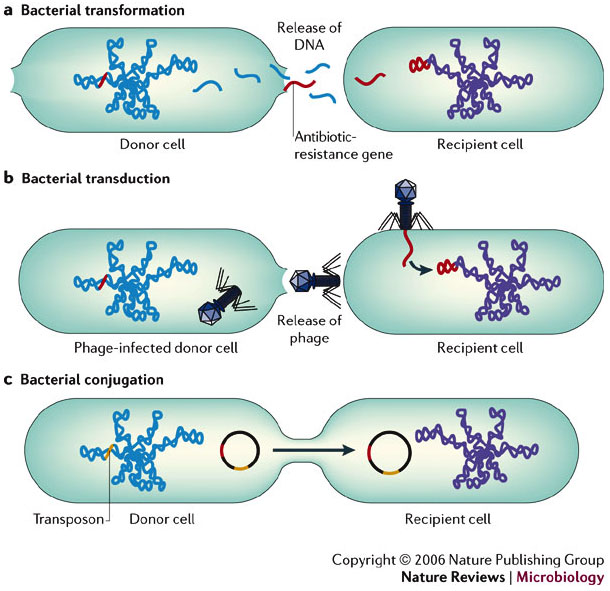
\includegraphics[scale=0.6]{hortran.jpg}
\caption{HGT Mechanisms}
\end{figure}
Each of these methods of genetic exchange can introduce sequences of DNA that share little homology with the remaining DNA of the recipient cell. If there are homologous sequences shared between the donor DNA and the recipient chromosome, the donor sequences can be stably incorporated into the recipient chromosome by genetic recombination. If the homologous sequences flank sequences that are absent in the recipient, the recipient may acquire an insertion from another strain of unrelated bacteria. Such insertions can be small or quite large. Large insertions that have been acquired from another bacterium (often inferred from differences in GC content or codon usage) and are absent from related strains of bacteria are called ``islands".\\

HGT is beneficial to a cell if the acquired gene confers a useful function, but is detrimental if the gene has no function, if it is incompatible with existing genes, or if it is a selfishly replicating mobile element. If the balance of these effects is beneficial on average, we would expect cells to evolve high rates of acceptance of horizontally transferred genes, whereas if it is detrimental, cells should reduce the rate of HGT as far as possible. It has been proposed that the rate of HGT was very high in the early stages of prokaryotic evolution, and hence there were no separate lineages of organisms. Only when the HGT rate began to fall, would lineages begin to emerge with their own distinct sets of genes. Evolution would then become more tree-like. This phenomenon has been called the Darwinian Threshold.

\end{document}